%% abtex2-modelo-trabalho-academico.tex, v-1.9.6 laurocesar
%% Copyright 2012-2016 by abnTeX2 group at http://www.abntex.net.br/ 
%%
%% This work may be distributed and/or modified under the
%% conditions of the LaTeX Project Public License, either version 1.3
%% of this license or (at your option) any later version.
%% The latest version of this license is in
%%   http://www.latex-project.org/lppl.txt
%% and version 1.3 or later is part of all distributions of LaTeX
%% version 2005/12/01 or later.
%%
%% This work has the LPPL maintenance status `maintained'.
%% 
%% The Current Maintainer of this work is the abnTeX2 team, led
%% by Lauro César Araujo. Further information are available on 
%% http://www.abntex.net.br/
%%
%% This work consists of the files abntex2-modelo-trabalho-academico.tex,
%% abntex2-modelo-include-comandos and abntex2-modelo-references.bib
%%

% ------------------------------------------------------------------------
% ------------------------------------------------------------------------
% abnTeX2: Modelo de Trabalho Academico (tese de doutorado, dissertacao de
% mestrado e trabalhos monograficos em geral) em conformidade com 
% ABNT NBR 14724:2011: Informacao e documentacao - Trabalhos academicos -
% Apresentacao
% ------------------------------------------------------------------------
% ------------------------------------------------------------------------

% ------------------------------------------------------------------------
% ------------------------------------------------------------------------
% C3FURG: Modelo de Trabalho Academico (tese de doutorado, dissertacao
% de mestrado e trabalhos monograficos em geral) do Centro de Ciencias
% Computacionais (C3) da Universidade Federal de Rio Grande (FURG) em
% conformidade com ABNT NBR 14724:2011: Informacao e documentacao -
% Trabalhos academicos - Apresentacao
% ------------------------------------------------------------------------
% ------------------------------------------------------------------------


\documentclass[
	% -- opções da classe memoir --
	12pt,				% tamanho da fonte
	%openright,			% capítulos começam em pág ímpar (insere página vazia caso preciso)
	%twoside,			% para impressão em recto e verso. Oposto a oneside
	a4paper,			% tamanho do papel. 
	% -- opções da classe abntex2 --
	%chapter=TITLE,		% títulos de capítulos convertidos em letras maiúsculas
	%section=TITLE,		% títulos de seções convertidos em letras maiúsculas
	%subsection=TITLE,	% títulos de subseções convertidos em letras maiúsculas
	%subsubsection=TITLE,% títulos de subsubseções convertidos em
        %letras maiúsculas
	% -- opções da classe C3FURG --
        ec,         % ec, si, ea, mestrado
        pgii,       %,ti, dm, dd % tipo de documento
	% -- opções do pacote babel --
	english,			% idioma adicional para hifenização
	%french,				% idioma adicional para hifenização
	%spanish,			% idioma adicional para hifenização
	brazil				% o último idioma é o principal do documento
	]{C3FURG}

% ---
% Pacotes básicos 
% ---
\usepackage{lmodern}			% Usa a fonte Latin Modern			
\usepackage[T1]{fontenc}		% Selecao de codigos de fonte.
\usepackage[utf8]{inputenc}		% Codificacao do documento (conversão automática dos acentos)
\usepackage{lastpage}			% Usado pela Ficha catalográfica
\usepackage{indentfirst}	  	        % Indenta o primeiro parágrafo de cada seção.
\usepackage{color}				% Controle das cores
\usepackage{graphicx}			% Inclusão de gráficos
\usepackage{microtype} 			% para melhorias de justificação
\usepackage{color,soul}
\usepackage{amsthm}
% ---
		
% ---
% Pacotes adicionais, usados apenas no âmbito do Modelo Canônico do C3FURG
% ---
\usepackage{lipsum}				% para geração de dummy text
% ---

% ---
% Pacotes de citações
% ---
\usepackage[brazilian,hyperpageref]{backref}	 % Paginas com as citações na bibl
\usepackage[alf]{abntex2cite}	% Citações padrão ABNT

% --- 
% CONFIGURAÇÕES DE PACOTES
% --- 

% ---
% Configurações do pacote backref
% Usado sem a opção hyperpageref de backref
\renewcommand{\backrefpagesname}{Citado na(s) página(s):~}
% Texto padrão antes do número das páginas
\renewcommand{\backref}{}
% Define os textos da citação
\renewcommand*{\backrefalt}[4]{
	\ifcase #1 %
		Nenhuma citação no texto.%
	\or
		Citado na página #2.%
	\else
		Citado #1 vezes nas páginas #2.%
	\fi}%
% ---

% ---
% Informações de dados para CAPA e FOLHA DE ROSTO
% ---
\titulo{Proposta de um modelo preditivo de tentativa de suicídio para usuários de drogas utilizando técnicas de Mineração de Dados \\ Universidade Federal do Rio Grande}
\autor{Vinicius Lucena dos Santos}
\local{Brasil}
\data{2018}
\orientador{Eduardo Nunes Borges}
\instituicao{%
  Universidade Federal do Rio Grande -- FURG
  \par
  Centro de Ciências Computacionais
  \par
  Curso de Engenharia de Computação}
\tipotrabalho{Projeto de Graduação}
% O preambulo deve conter o tipo do trabalho, o objetivo, 
% o nome da instituição e a área de concentração 


\preambulo{Trabalho acadêmico apresentado ao Curso de Engenharia de
   Computação da Universidade Federal do Rio Grande como requisito
   parcial para a obtenção do grau de Bacharel em Engenheira de Computação.}
   
% -- Definições -- %
\newtheorem{definition}{Definição}



% ---
% Configurações de aparência do PDF final

% alterando o aspecto da cor azul
\definecolor{blue}{RGB}{41,5,195}

% informações do PDF
\makeatletter
\hypersetup{
  % pagebackref=true,
  pdftitle={\@title}, 
  pdfauthor={\@author},
  pdfsubject={\imprimirpreambulo},
  pdfcreator={LaTeX with C3FURG},
  pdfkeywords={palavra-chave1}{palavra-chave2}{palavra-chave3}{palavra-chave4}, 
  colorlinks=true,       		% false: boxed links; true: colored links
  linkcolor=blue,          	        % color of internal links
  citecolor=blue,        		% color of links to bibliography
  filecolor=magenta,      		% color of file links
  urlcolor=blue,
  bookmarksdepth=4
}
\makeatother
% --- 

% --- 
% Espaçamentos entre linhas e parágrafos 
% --- 

% O tamanho do parágrafo é dado por:
\setlength{\parindent}{1.3cm}

% Controle do espaçamento entre um parágrafo e outro:
\setlength{\parskip}{0.2cm}  % tente também \onelineskip

% ---
% compila o indice
% ---
\makeindex
% ---

% ----
% Início do documento
% ----
\begin{document}

% Seleciona o idioma do documento (conforme pacotes do babel)
%\selectlanguage{english}
\selectlanguage{brazil}

% Retira espaço extra obsoleto entre as frases.
\frenchspacing 

% ----------------------------------------------------------
% ELEMENTOS PRÉ-TEXTUAIS
% ----------------------------------------------------------
% \pretextual

% ---
% Capa
% ---
\imprimircapa
% ---

% ---
% Folha de rosto
% (o * indica que haverá a ficha bibliográfica) - APENAS NA VERSÃO FINAL
% ---
\imprimirfolhaderosto
% ---


% ---
% RESUMOS
% ---
% resumo em português
\setlength{\absparsep}{18pt} % ajusta o espaçamento dos parágrafos do resumo
\begin{resumo}
 Texto do resumo em português.

 \textbf{Palavras-chave}: palavra-chave 1. palavra-chave 2. palavra-chave 3.
\end{resumo}

% resumo em inglês
\begin{resumo}[Abstract]
 \begin{otherlanguage*}{english}
   This is the english abstract.

   \textbf{Keywords}: keyword 1. keyword 2. keyword 3.
 \end{otherlanguage*}
\end{resumo}



% ---
% inserir lista de ilustrações
% ---
\pdfbookmark[0]{\listfigurename}{lof}
\listoffigures*
\cleardoublepage
% ---

% ---
% inserir lista de tabelas
% ---
\pdfbookmark[0]{\listtablename}{lot}
\listoftables*
\cleardoublepage
% ---

% ---
% inserir lista de abreviaturas e siglas
% ---
\begin{siglas}
  \item[KDD] Knowledge Discovery in Database
\end{siglas}
% ---

% ---
% inserir lista de símbolos
% ---
\begin{simbolos}
  \item[$ \Gamma $] Letra grega Gama
  \item[$ \Lambda $] Lambda
  \item[$ \zeta $] Letra grega minúscula zeta
  \item[$ \in $] Pertence
\end{simbolos}
% ---

% ---
% SUMÁRIO
% ---
\pdfbookmark[0]{\contentsname}{toc}
\tableofcontents*
\cleardoublepage
% ---



% ----------------------------------------------------------
% ELEMENTOS TEXTUAIS
% ----------------------------------------------------------
% ---
% INTRODUÇÃO
% ---
\chapter{Introdução}
\label{cap:introducao}

De acordo com um estudo realizado pela Organização Mundial da Saúde em 2014, mais de 1 milhão de pessoas tiram a própria vida por ano, é a segunda maior causa de mortes entre jovens de 15 a 29 anos de idade. No Brasil, em média, o número de suicídio é de 11 mil por ano, sendo a quarta maior causa de mortes entre os jovens do sexo masculino. Considerando apenas o grupo etário mais economicamente produtivo (15-44 anos), o suicídio é uma das três causas principais causa de morte em todo mundo, dessa forma, nota-se que também há impactos econômicos no ato de tirar a própria vida. 

Segundo um estudo realizado pelo Ministério da Saúde, o número de suicídios no Brasil aumentou durante 16 anos consecutivos, entre os anos de 2000 a 2016. Os principais fatores de risco para o suicídio incluem doença mental ou física, abuso de álcool e drogas, mudança súbita na vida, como a perda de emprego, término de um casamento ou a combinação desses com outros acontecimentos. Para os amigos e familiares do suicida, o impacto é significativo, tanto imediatamente quanto a longo prazo. 

O Hospital das Clínicas de Porto Alegre (HCPA) é uma instituição pública e universitária, ligada ao Ministério da Educação e à Universidade Federal do Rio Grande do Sul (UFRGS).
A pesquisa produzida no HCPA, por sua vez, introduz novos conhecimentos, técnicas e tecnologias que beneficiam toda a sociedade, além de formar novas gerações de pesquisadores.

% ----------------------------------------------------------------------------------------
parágrafo 1: explicar o que são e como se relacionam: HCPA, UFRGS, Departamento de Psiquiatria e Medicina Legal, Programa de Pós-Graduação em Psiquiatria e Ciências do Comportamento, e o CPAD. Tem informações na Web e um resumo no texto do projeto enviado por email

parágrafo 2: resumir o projeto em que eu estou trabalhando com base no texto do projeto e no meu Plano de Trabalho enviados por email.

parágrafo 3: explicar que o foco do trabalho apresentado nesta monografia é contribuir com a construção dos modelos preditivos de tentativa de suicídio.
% ----------------------------------------------------------------------------------------


\section{Objetivos}
\label{sec:objetivos}
O principal objetivo do atual projeto é utilizar técnicas de mineração de dados para criar um modelo preditivo a fim de predizer se um determinado paciente tentará cometer suicídio ou não. 

Como objetivo específico pretende-se descobrir os atributos que mais influenciam na tentativa de um suicídio.

\section{Estrutura da monografia}

% ---

% ---
% FUNDAMENTAÇÃO
% ---
\chapter{Fundamentação Teórica}
Este capítulo aborda a fundamentação teórica necessária para o profundo entendimento do presente trabalho, bem como do modelo de classificação proposto. Primeiramente é introduzido o conceito de Descoberta de Conhecimento em Banco de Dados. Após, é detalhado o conceito e funcionamento de três algoritmos usados para classificação, são eles: Florestas Aleatórias, Support Vector Machine e Adaboost. 

% --- Descoberta de Conhecimento em Banco de Dados --- %
\section{Descoberta de Conhecimento}
A primeira vez que apareceu o termo \textit{Descoberta de Conhecimento em Banco de Dados} (do inglês \textit{Knowledge Discovery in Database}) foi em 1989, por Piatetsky-Shapiro, com o objetivo de enfatizar que o produto final do processo é o conhecimento.

Para \cite{fayyad:1996} KDD refere-se ao processo geral de descobrir conhecimento útil a partir dos dados, essa extração de conhecimento é um processo não-trivial. 
A Figura ~\ref{fig:kdd} mostra o processo de KDD proposto por Fayyad et al. 
O termo processo implica que o KDD é composto por várias etapas, as quase são iterativas e interativas. 
Iterativa reflete o ciclo entre as etapas e, interativa reflete o caráter interdisciplinar do processo, uma vez que o KDD se aplica em inúmeras áreas e para resolver o problema muitas vezes é necessária a ajuda de um \textit{expert} naquela área.

A seguir, será dada uma visão geral de cada uma das fases.


\begin{figure}
    \centering
    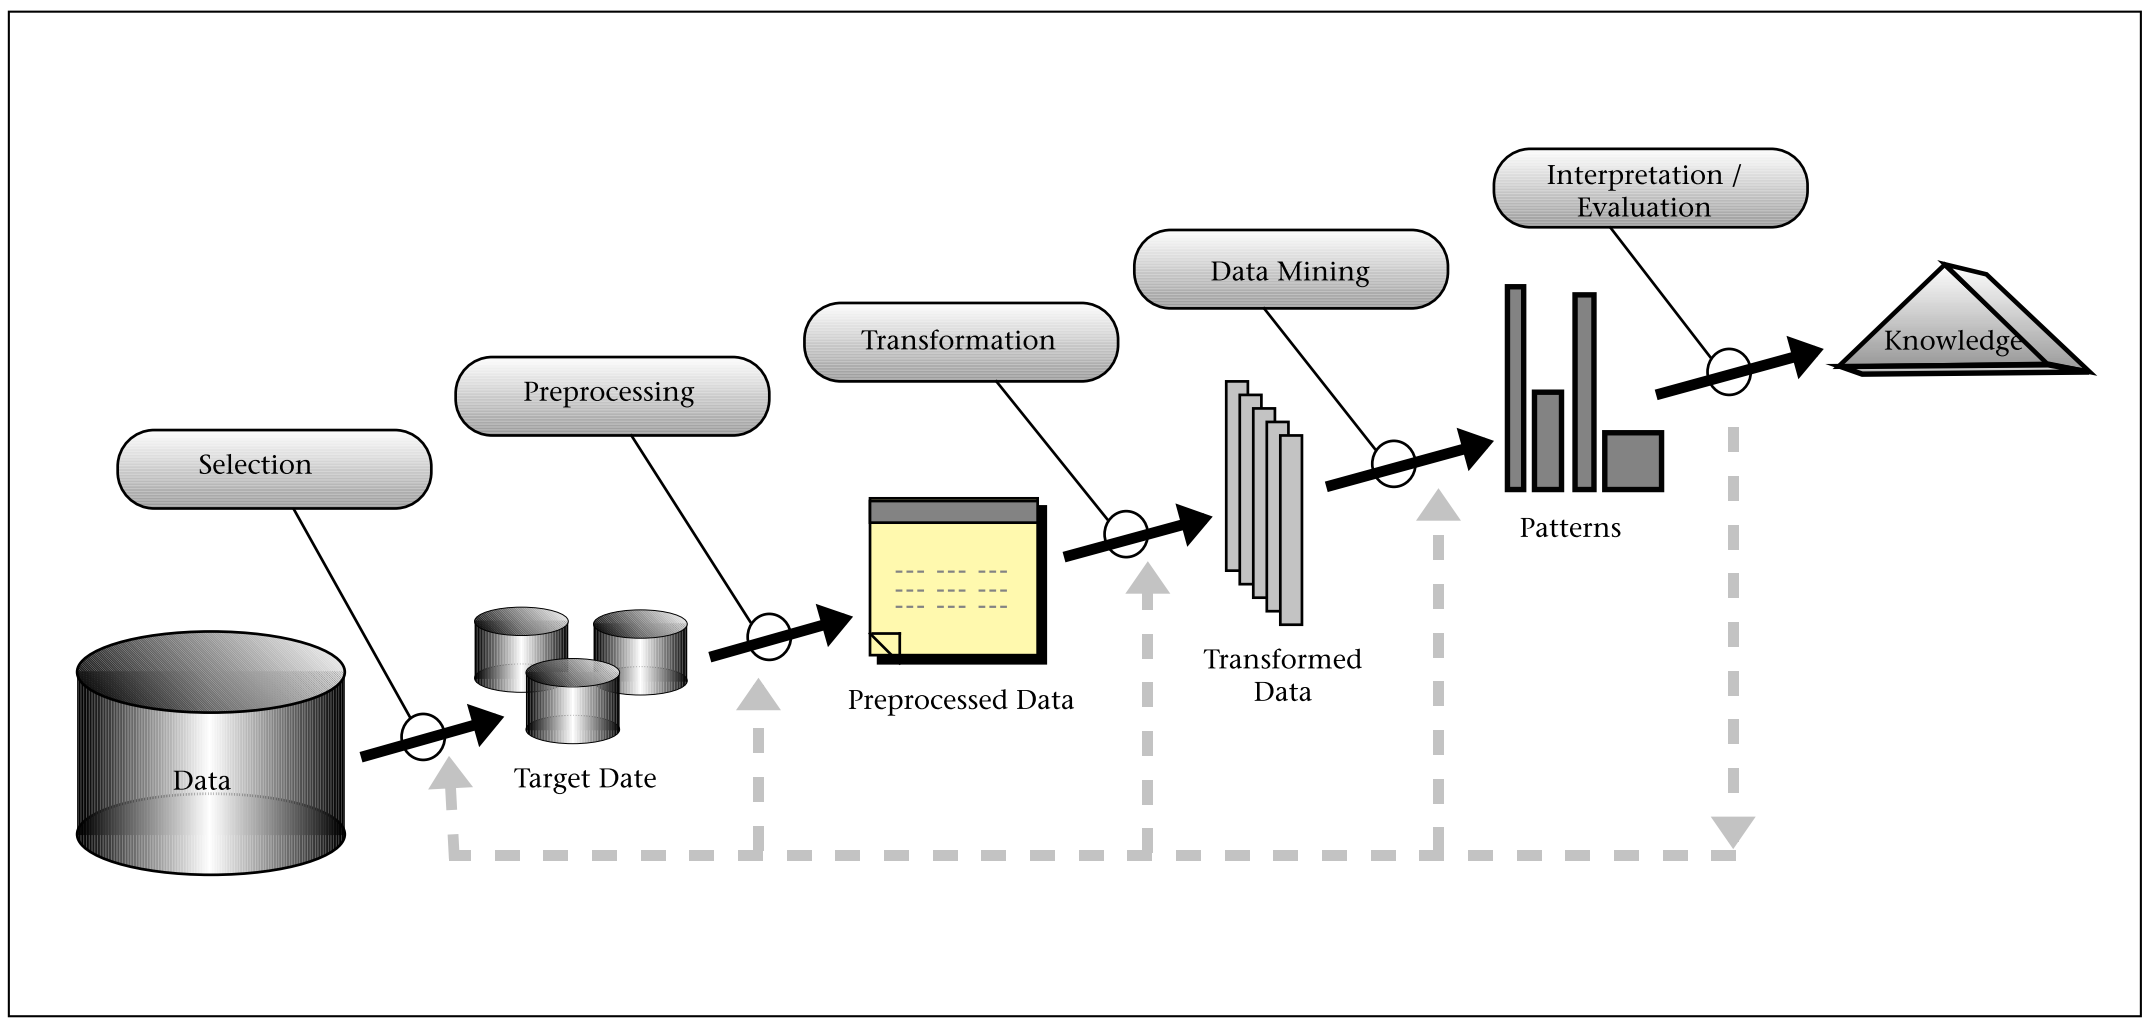
\includegraphics[scale=0.39]{Imagens/kdd.png}
    \caption{Processo de KDD (Fayyad et al)}
    \label{fig:kdd}
\end{figure}

\subsection{Fases do KDD}
% --- SELEÇÃO --- %
\textbf{1) Seleção}: A primeira etapa no processo é chamada de seleção, que é responsável por selecionar um \textit{dataset} a partir de uma base de dados maior. A escolha desse \textit{dataset} dependerá do domínio do problema que está tentando resolver. Em geral, a escolha é feita por um especialista ou por algum algoritmo de extração de características. O conjunto de dados selecionado é chamado de \textit{Target Data}.

% --- PRÉ-PROCESSAMENTO -- %
\textbf{2) Pré-processamento}: Após ter o conjunto de dados a ser utilizado, é comum que esses dados não estejam em boa qualidade, dessa forma, é necessário tratá-los e limpá-los. Operações básicas realizadas nesse nível devem lidar com:

\begin{itemize}[leftmargin=1.2cm]
%    \begin{description}[font=$ \bullet $]
        \item [ Valores faltantes] Valores nulos. Ocorre quando alguém deixa um campo de um formulário em branco, por exemplo.
        \item [ \textit{Outliers}] Quando um valor foge muito do padrão dos dados. Deve ser identificado e eliminado do conjunto de dados.
        \item[ Dados derivados] Ocorre quando um dado pode ser obtido a partir de outro. Por exemplo, a idade de um indivíduo pode ser obtida a partir do seu ano de nascimento, dessa forma, não faz muito sentido ter esses dois atributos no conjunto de dados.
 %   \end{description}
\end{itemize}

% --- TRANSFORMAÇÃO -- %
\textbf{3) Transformação}: Uma vez que os dados estão limpos e tratados, é necessário armazená-los e formatá-los adequadamente para que os algoritmos de aprendizado possam ser utilizados. A título de exemplo, se for usar um algoritmo de agrupamento baseado na distância euclidiana, é necessário converter todos os dados para numérico.

% --- MINERAÇÃO DE DADOS -- %
\textbf{4) Mineração de Dados}:  Embora todas as etapas sejam importantes, a etapa de Mineração de Dados é a que recebe maior atenção. Conforme \cite{fayyad:1996}, mineração de dados é a aplicação de algoritmos específicos para extrair padrões a partir dos dados. Ainda de acordo com Fayyad et al, os algoritmos de mineração de dados podem ser dividimos em cinco categorias: Associação, Classificação, Regressão, Segmentação e Sumarização. A tarefa na qual este projeto se encontra é a de classificação. 

A tarefa de classificação é responsável por identificar a qual classe um determinado registro pertence. Inicialmente, o modelo é ``alimentado'' com conjunto de registros já rotulados, isto é, é fornecida a qual classe os registros pertencem. Com esses dados, o algoritmo treina a aprende padrões que fazem com que um registro pertença a uma classe ou a outra
(esse tipo de aprendizado é conhecido como aprendizado supervisionado).


% -- INTERPRETAÇÃO/VALIDAÇÃO -- %
\textbf{5) Interpretação/Validação}: Uma vez que o modelo já foi treinado, é medido a sua capacidade de generalização. Nesta etapa é fundamental a presença do especialista, visto que, a melhor métrica de avaliação dependerá do negócio. Caso o desempenho não seja satisfatório, é possível retornar para qualquer etapa no processo de KDD, e o ciclo recomeça até chegar a um modelo que satisfaça o negócio.







% --- Ensemble --- %
\section{Ensemble Learning}
\label{sec:ensemble}
Um \textit{ensemble} é composto por um grupo de preditores, que nada mais são do que algoritmos de aprendizado de máquina supervisionados. A técnica de combinar vários preditores é conhecida como \textit{Ensemble Learning} \cite{Geron:2017}. Existem vários métodos baseados nessa estratégia, os mais conhecidos na literatura são: \textit{bagging}, \textit{boosting} e \textit{stacking}.

A figura \ref{fig:ensemble} ilustra um \textit{ensemble} composto por quatro preditores, dos quais três predizeram que uma nova instância é da classe 1 e um preditor disse que a nova instância é da classe 2. Como neste caso, o \textit{ensemble} escolhe a classe de acordo com a votação majoritária de seus preditores, é atribuída a classe 1 à nova instância.

\begin{figure}[ht!]
    \centering
    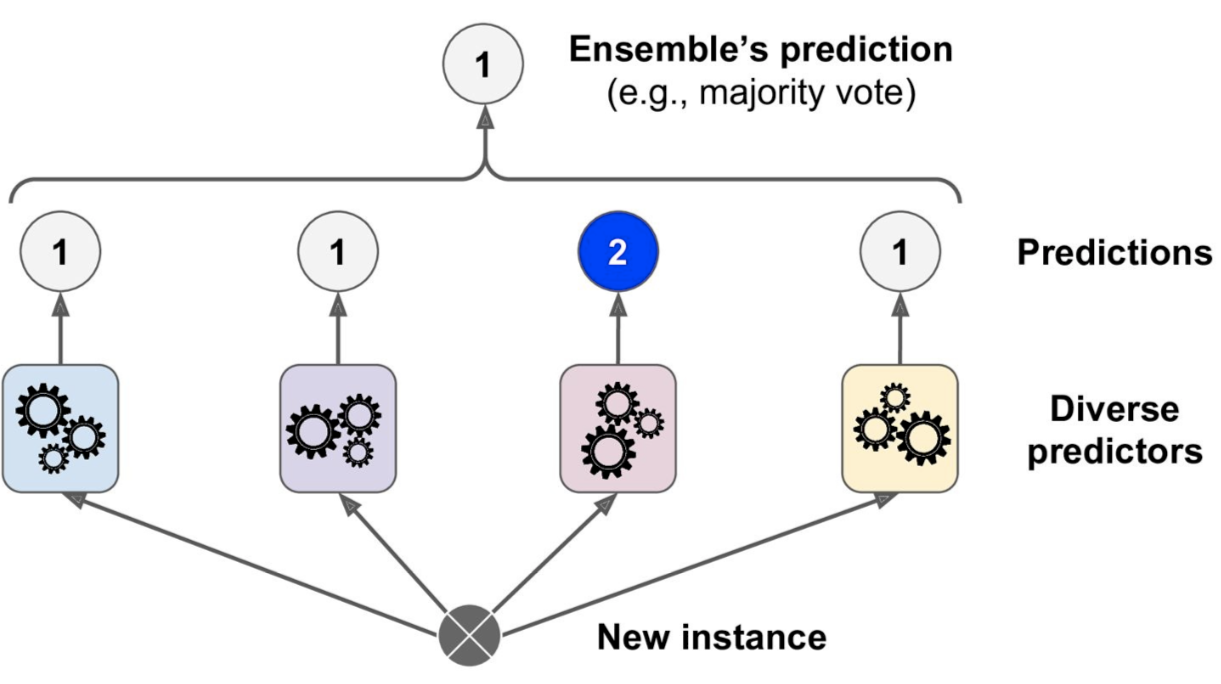
\includegraphics[scale=0.2]{Imagens/ensemble.png}
    \caption{Exemplo de um Ensemble Learning \cite{Geron:2017}}
    \label{fig:ensemble}
\end{figure}

Embora seja mais comum utilizar \textit{Ensemble Learning} para classificação, também é possível utilizar essa técnica para problemas de regressão.

Uma maneira muito simples de agregar os resultados de cada preditor, a fim de chegar em um classificar ainda mais robusto, é escolher a classe com a maior quantidade de votos. Essa estratégia é conhecida como \textit{Hard Voting Classifier} \cite{Geron:2017}.

Contudo, é possível que haja classificadores bons e ruins, caso o número de preditores ruins supere o número de bons, é possível que o método \textit{ensemble} seja prejudicado e tenha um resultado inferior ao melhor preditor. Para contornar esse tipo de problema, uma estratégia possível é atribuir pesos diferentes para os preditores, essa estratégia é conhecida como \textit{Soft Voting Classifier} \cite{Geron:2017}.


\subsection{Bagging e Pasting}
\label{sec:bagging_pasting}
Quando for construir um modelo \textit{ensemble}, uma abordagem possível é utilizar o mesmo algoritmos para treinar os preditores. Contudo, caso os preditores sejam treinados com o mesmo \textit{dataset}, todos os preditores terão o mesmo desempenho, dessa forma, é necessário que os preditores sejam treinados com uma amostra aleatória do conjunto de dados. Caso a amostragem seja feita \textit{com reposição}, esse método é chamado de \textit{bagging} \cite{Breiman_Bagging:1996}. Caso a amostragem seja feita \textit{sem reposição}, o método é chamado de \textit{pasting} \cite{Breiman_Pasting:1999}. 

% --- Florestas Aleatórias --- %
\section{Florestas Aleatórias}

Florestas Aleatórias (do inglês \textit{Random Forest}) é um algoritmo de aprendizado do tipo \textit{ensemble} cujo os meta-classificadores são Árvores de Decisão \cite{Quinlan:1986} treinadas com o método \textit{bagging}.
De acordo com \cite{breiman:2001} a definição formal do algoritmo Floresta Aleatória é dada por:

\begin{definition}\label{def:floresta}
Uma floresta aleatória é um classificador que consiste em uma coleção de classificadores de árvores de decisão ${h(x, \theta _k)}$, onde ${\theta _k}$ são as \textit{features} para o meta-classificador $k$ e, $x$ é o vetor de entrada.
\end{definition}

O algoritmo de Floresta Aleatória introduz um certo nível de aleatoriedade ao treinar os meta-classificadores; em vez de receberem o mesmo conjunto de dados, as árvores de decisão recebem um subconjunto diferente. Por exemplo, na figura \ref{fig:split_floresta} o \textit{dataset} original foi dividido em 2 subconjuntos de dados, os quais serão utilizados para treinar os algoritmos de árvore de decisão. Nota-se que as \textit{features} escolhidas não são as mesmas. Esse processo é importante, pois aumenta a capacidade de generalização do modelo de classificação.

\begin{figure}[h!]
    \centering
    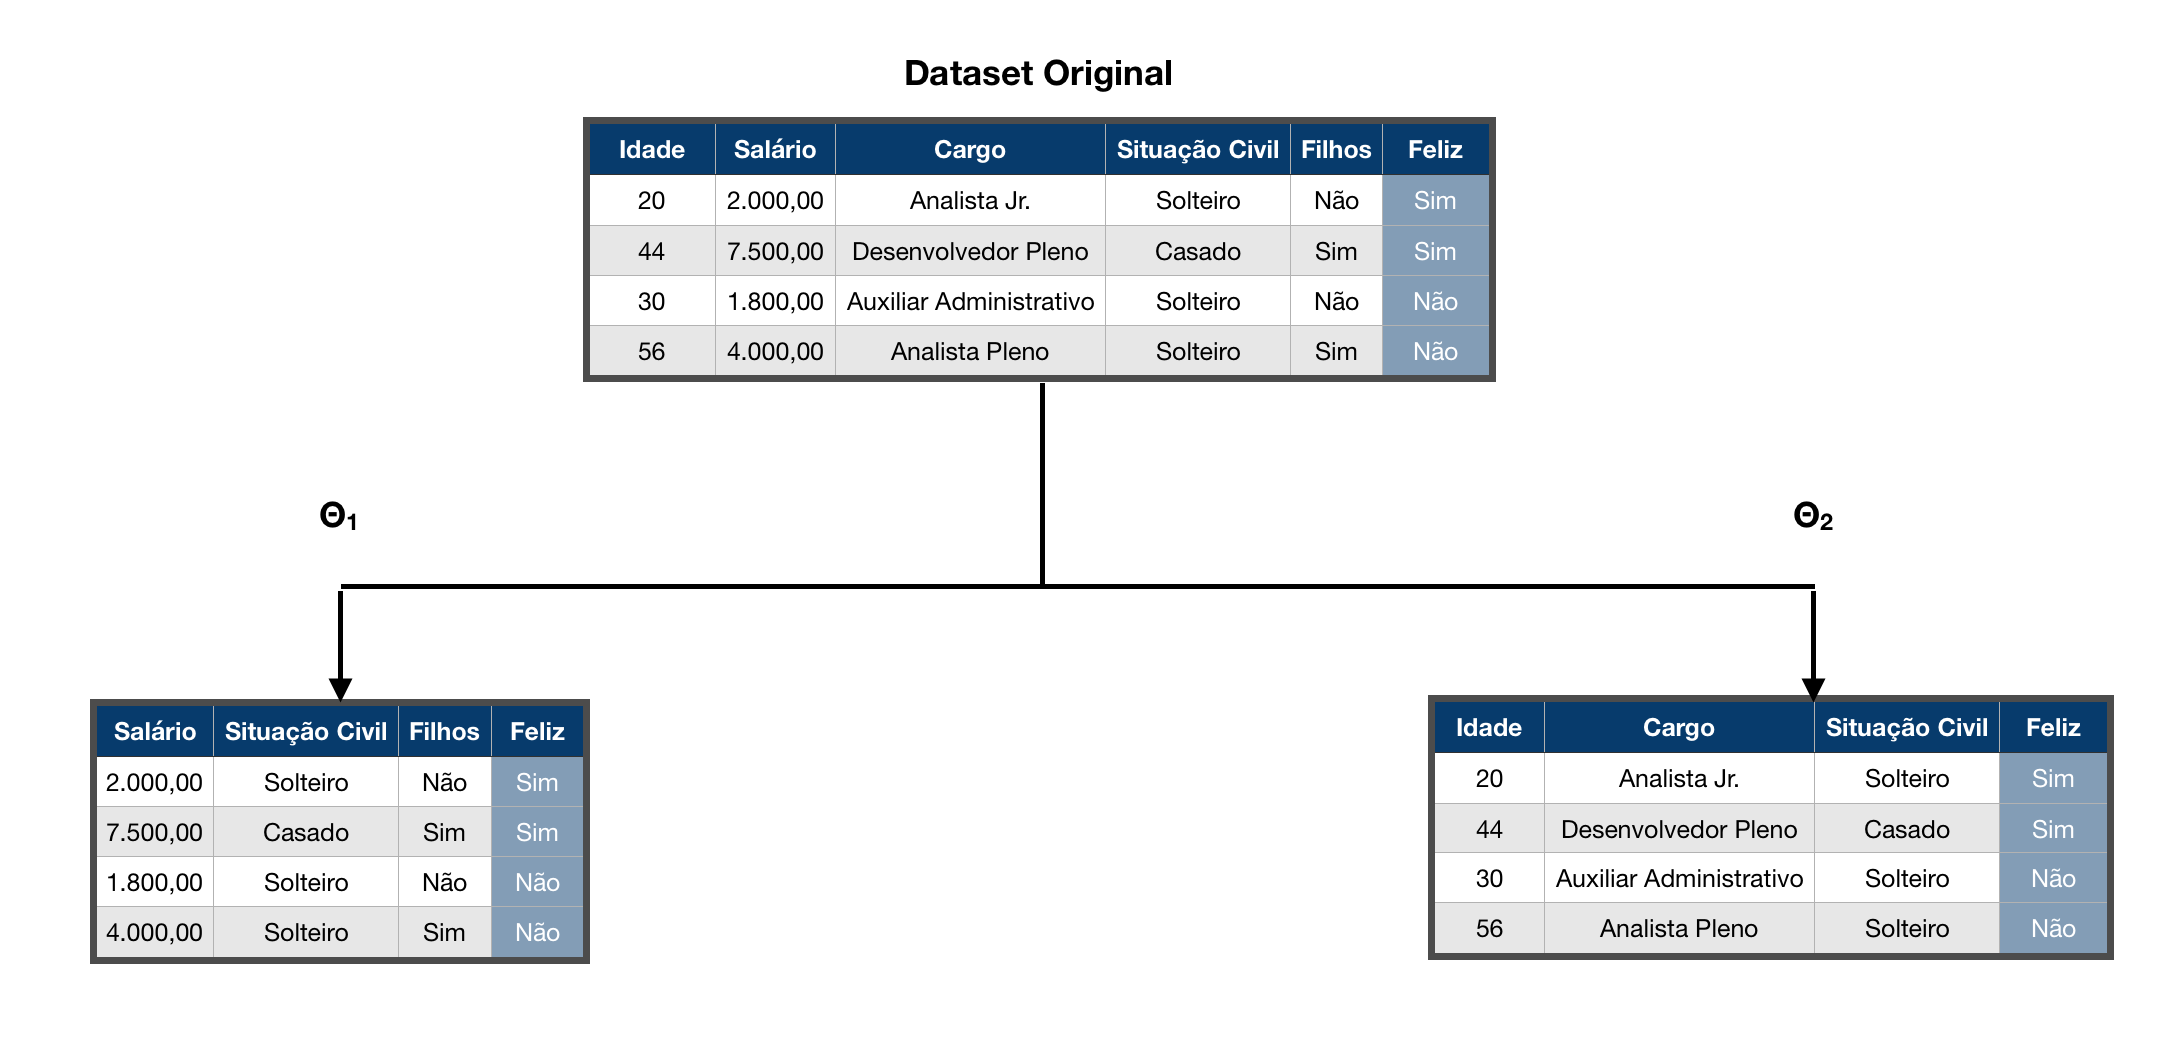
\includegraphics[scale=0.4]{Imagens/split_RandomForest.png}
    \caption{Exemplo de uma divisão randômica do \textit{dataset} original.}
    \label{fig:split_floresta}
\end{figure}

\subsection{A importância das features}
\label{sec:importancia_features}
Uma grande qualidade das florestas aleatórias é o fato de ser possível identificar as melhores \textit{features}, em outras palavras, é possível saber quais são os atributos mais importantes para predizer se um determinado registro irá pertencer a uma classe ou a outra. Se o modelo está sendo treinado para identificar uma doença de acordo com os sintomas, é possível descobrir quais são os sintomas que mais influenciam em um paciente possuir uma determinada doença.


\subsection{Vantagens e Desvantagens}
Um ponto positivo das Florestas Aleatórias é que esse tipo de algoritmo pode ser usado tanto para problemas de classificação quanto para problemas de regressão. 

Como foi dito na sessão \ref{sec:importancia_features}, é possível visualizar a importância de cada \textit{feature}, a fim de compreender melhor o comportamento dos dados e interpretar o modelo aprendido.

Um grande problema que aflige alguns algoritmos de aprendizado supervisionado é o \textit{overfitting}, isto ocorre quando um modelo aprende muito bem o conjunto de treino e sua capacidade de generalização fica comprometida por conta disso. Na maioria das vezes, esse problema não irá acontecer com o modelo de Floresta Aleatória.

A grande desvantagem do modelo de Floresta Aleatória fica por conta da sua performance quando há uma grande quantidade de árvores. Por um lado, quanto mais meta-classificadores melhor tende a ser a acurácia do modelo. Por outro lado, se há muitos meta-classificadores, a performance do algoritmo fica bastante comprometida.

% --- Adaboost --- %
\section{AdaBoost}

O modelo \textit{boosting} refere-se a um método \textit{ensemble} (sessão \ref{sec:ensemble}) para resolver problemas de classificação e regressão. A ideia geral do \textit{boosting} é  combinar vários meta-algoritmos fracos em um modelo robusto. Esses meta-algoritmos são treinados em sequência, onde cada um tenta corrigir seu antecessor \cite{Kearns:1988}.

O algoritmo do tipo \textit{boosting} mais conhecido na literatura é o \textit{Adaptive Boosting} ou simplesmente \textit{AdaBoost}, que foi proposto por \cite{Freund:1997}. O algoritmo pode ser usado para melhorar o desempenho de qualquer algoritmo de \textit{machine learning}. Contudo, AdaBoost funciona melhor com preditores fracos \footnote{Preditores fracos são aqueles que alcançam uma acurácia pouco acima de um preditor aleatório.}.

O preditor mais comum para ser usado com o AdaBoost são as árvores de decisão com um nível. Pelo fato dessas árvores possuírem apenas um nível, são conhecidas na literatura como \textit{Decision Stump} (algo como Toco de Decisão, em vez de Árvore de Decisão).

\subsection{Funcionamento}
O trabalho de \cite{Freund:1999} foi utilizado como referência para a explicação do funcionamento do algoritmo que será dada a seguir.

Inicialmente, é fornecido como entrada para o algoritmo, o conjunto de treino $(x_1, y_1), (x_2, y_2) ..., (x_m, y_m)$, onde cada $x_i$ pertence ao conjunto de instâncias $X$, e cada $y_i$ pertence ao conjunto de rótulos $Y$. Para problemas envolvendo a classificação binária (ou dicotômica), considera-se $Y = \{-1, +1\}$. 

Adaboost utiliza $T$ preditores, os autores chamam os preditores de \textit{hipóteses}, denotando as hipóteses como sendo $h_1(x), h_2(x),..., h_T(x)$, onde $x$ representa uma instância a ser classificada pela hipótese (preditor) $h_t(x)$.

Uma das principais ideias do algoritmo é manter uma distribuição ou conjunto de
pesos sobre o conjunto de treinamento. Isto é, cada instância no conjunto de treinamento existe um peso associado e, a medida que o algoritmo evolui, quanto mais difícil for para classificar uma instância de treinamento, maior será o peso atribuído a ela. De modo que, para os preditores subsequentes, a chance de classificar corretamente esse dado é maior. O peso dessa distribuição para um dado de treinamento $i$ na rodada $t$ é denotado por $D_t(i)$.

Inicialmente, todas as instâncias no conjunto de treinamento possuem exatamente o mesmo peso $w_i = \dfrac{1}{N}$, onde $N$ é o tamanho do conjunto de treinamento. Mas, a cada rodada, o peso das amostras classificadas erroneamente são aumentados, dessa forma, os preditores são forçados a focar nas amostras mais difíceis de serem classificadas.




% --- Support Vector Machine --- %
\section{SVM}

Máquinas de Vetores de Suporte, do inglês \textit{Support Vector Machines}, é um tipo de algoritmo de Aprendizado de Máquina supervisionado, utilizado para problemas de classificação envolvendo duas ou mais classes. O algoritmo foi proposto por \cite{Cortes:1995}. 

A ideia do SVM é mapear vetores de entrada em alguma dimensão maior, através de algum mapeamento não-linear, escolhido a piori. Neste novo espaço um hiperplano é construído para separar os dados \cite{Cortes:1995}.

\begin{figure}[ht!]
    \centering
    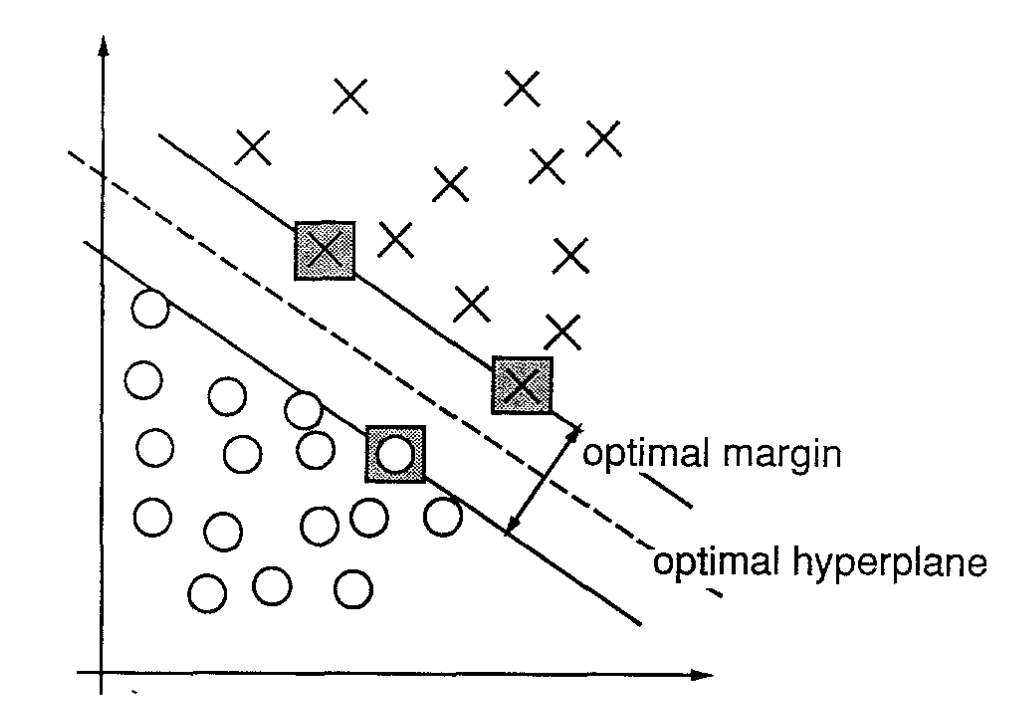
\includegraphics[scale=0.70]{Imagens/svm-exemplo.png}
    \caption{Um exemplo de um conjunto de dados linearmente separável em duas dimensões. \cite{Cortes:1995}}
    \label{fig:svm-exemplo}
\end{figure}

A figura \ref{fig:svm-exemplo} mostra um conjunto de dados que pode ser separado de maneira linear. O objetivo do SVM é encontrar o melhor hiperplano, de maneira que a margem\footnote{Margem é o dobro da distância entre o hiperplano e o ponto mais perto} seja a maior possível. 

\subsection{Vantagens e Desvantagens}
Um \textit{Support Vector Machine} é um modelo de classificação poderoso e versátil, capaz de realizar classificação linear e não linear, regressão e até detecção de \textit{outliers}. SVMs são parcularmente bem adequadas para problemas de classificação complexo, porém com \textit{datasets} não muito grandes \cite{Geron:2017}.

Um lado negativo do SVM é sua sensibilidade à escala dos dados de entrada. A figura \ref{fig:svm-escala} ilustra bem esse problema: no desenho da esquerda, aonde $x_0$ e $x_1$ estão em escalas diferentes, a margem é bem pequena. Quando os dados são normalizados, como mostra no desenho da direita, a margem fica bem maior, possibilitando melhor generalização na hora de classificar novas instâncias.

\begin{figure}[ht!]
    \centering
    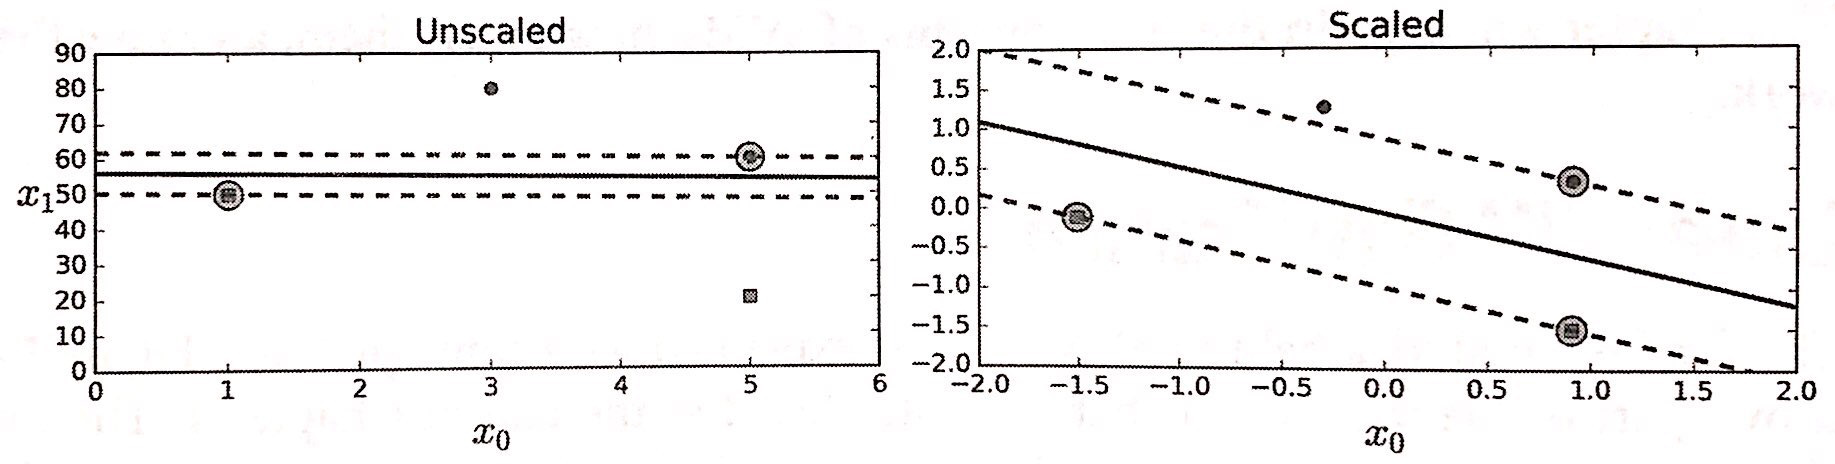
\includegraphics[scale=0.25]{Imagens/smv_escala.png}
    \caption{Sensibilidade com a escala dos dados \cite{Geron:2017}}
    \label{fig:svm-escala}
\end{figure}


% ---

% ---
% METODOLOGIA
% ---
\chapter{Metodologia}

Lorem ipsum dolor sit amet, consectetur adipiscing elit. Aliquam hendrerit malesuada laoreet. In hac habitasse platea dictumst. Vestibulum et erat elit. Quisque tempor dui id est lacinia, ut gravida nulla lacinia. Ut egestas varius nibh, ac ullamcorper nunc malesuada sit amet. Suspendisse fermentum condimentum elit, a fringilla leo molestie vel. Aenean ac quam sodales est tincidunt commodo at sit amet eros. Quisque in congue ligula, vel posuere purus. Vivamus sit amet ultricies elit.

Curabitur pellentesque volutpat ornare. Pellentesque pulvinar tincidunt ligula, vel lacinia augue iaculis consequat. Suspendisse sollicitudin tristique dictum. Cras vestibulum, felis consectetur euismod elementum, quam purus pellentesque diam, at convallis dui lectus imperdiet eros. Donec vitae turpis lacinia, auctor ligula id, tincidunt arcu. Nunc non rutrum nunc. Nam ornare est vitae elementum dignissim. Curabitur posuere arcu purus, vitae efficitur nibh bibendum ac. Maecenas convallis justo sit amet ullamcorper pellentesque. Cras non ante eleifend, consectetur risus lobortis, porta est. Morbi ac justo id erat placerat convallis. Class aptent taciti sociosqu ad litora torquent per conubia nostra, per inceptos himenaeos. Pellentesque et dolor scelerisque, lacinia ligula at, imperdiet purus.

Pellentesque vitae elit quis nulla lobortis eleifend ut quis felis. Donec nec feugiat turpis. Donec tincidunt id felis nec mattis. Donec vitae convallis libero. Praesent auctor nibh tortor, et egestas turpis ultricies id. Nunc nibh ipsum, iaculis a neque vitae, mollis congue nisi. Nulla facilisi. Vivamus massa nulla, lacinia sed nisl sit amet, varius convallis dui. In aliquam ut arcu non commodo.
% ---

% ---
% RESULTADOS ESPERADOS
% ---
\chapter{Resultados Esperados}

Neste capítulo são discutidos os resultados que são esperados até a conclusão desta monografia.

Como dito no capítulo \ref{cap:introducao}, o principal objetivo do atual projeto é utilizar técnicas de mineração de dados para criar um modelo preditivo a fim de predizer se um determinado paciente tentará cometer suicídio ou não. Sendo mais específico na definição do objetivo geral, o modelo de classificação esperado deve possuir a medida de acurácia acima de 0.80 com a revocação acima de 0.90.
% ---

% ---
% CRONOGRAMA
% ---
\chapter{Cronograma}
A figura \ref{fig:cronograma} descreve o cronograma de andamento do Projeto de Graduação.

\begin{figure}[h!]
    \centering
    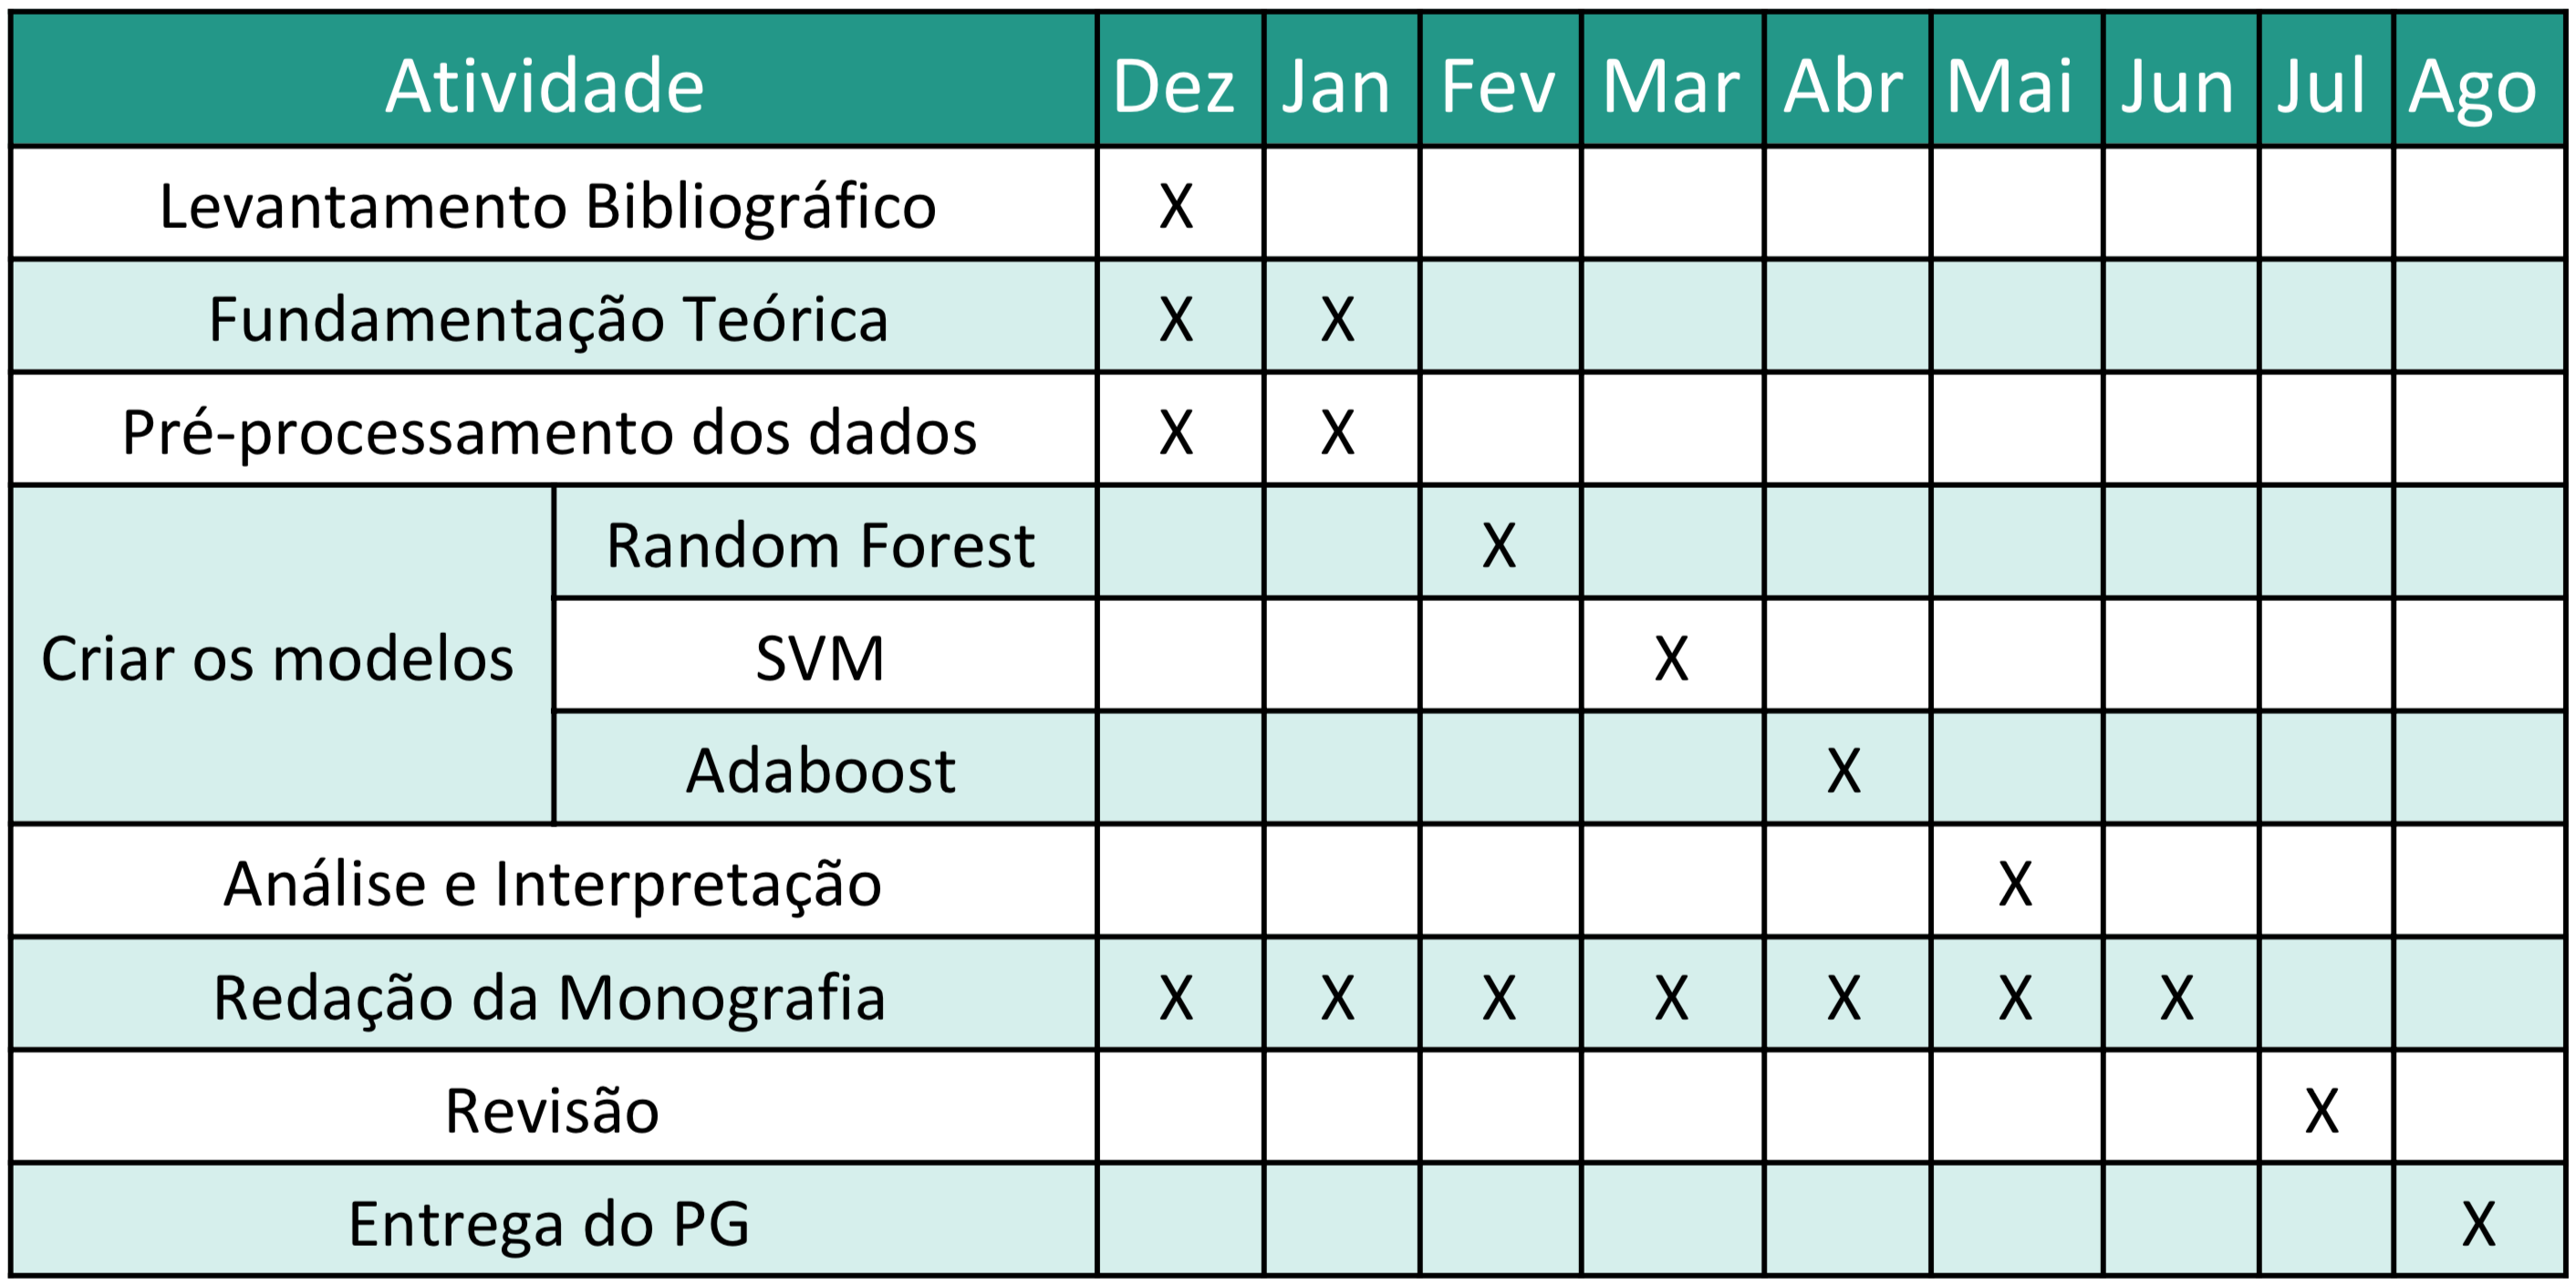
\includegraphics[scale=0.3]{Imagens/Cronograma.png}
    \caption{Cronograma}
    \label{fig:cronograma}
\end{figure}
% ---

% ----------------------------------------------------------
% Referências bibliográficas
% ----------------------------------------------------------
\bibliography{bibliografia}


\end{document}
